\begin{frame}{L'intégration}
    \begin{block}{Problème}
        Soit $\x(t)$ la position d’un objet rigide au temps $t$, $\v(t) =
        \dot{\x}(t)$ sa vélocité, et $\a$ son accélération constante.\\
        Trouver la position et la vélocité de l’objet au temps $t + \Delta t$.
    \end{block}
    \only<2>{
    \begin{itemize}
        \item Euler explicite (instable):
            \[
                \left\{
                \begin{array}{ccl}
                    \v(t + \Delta t) & = & \v(t) + \Delta t * \a\\
                    \x(t + \Delta t) & = & \x(t) + \Delta t * \v(t)\\
                \end{array}
                \right.
            \]
            \pause
        \item Euler semi-implicite (stable):
            \[
                \left\{
                \begin{array}{ccl}
                    \v(t + \Delta t) & = & \v(t) + \Delta t * \a\\
                    \x(t + \Delta t) & = & \x(t) + \Delta t * \v(t \textcolor{red}{+ \Delta t})\\
                \end{array}
                \right.
            \]
    \end{itemize}
    }
\end{frame}

\begin{frame}{La détection de collision}
    \begin{block}{Problème}
        Soient $n$ objets rigides. Trouver les points et normales de contact
        entre les objets qui se touchent.
    \end{block}
    \only<2>{
    \begin{figure}[h]
        \setcounter{subfigure}{0}
        \subfigure[Entrée]{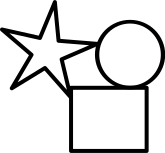
\includegraphics[height=.25\linewidth]{contact_nocontact}}
        \subfigure[Sortie]{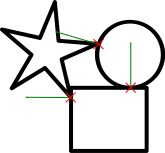
\includegraphics[height=.25\linewidth]{contact}}
    \end{figure}
    \pause
    \textbf{Il y a $n * (n - 1) / 2$ paires à tester en tout !}
    }
\end{frame}

\begin{frame}{La détection de collision}
    Que fait-on de ça ?
    \begin{center}
        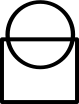
\includegraphics[scale=0.75]{penetration}
    \end{center}
    \pause
    \begin{itemize}
        \item On dit que les objets sont en \textbf{pénétration}.
            \pause
        \item La \textbf{pénétration}, c’est pas beau, et n’arrive jamais dans
            la vie réelle.
            \pause
        \item On mesure la \textbf{profondeur de pénétration} en plus du point
            de contact et de la normale.
    \end{itemize}
    \begin{center}
        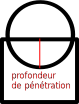
\includegraphics[scale=0.75]{penetration_depth}
    \end{center}
\end{frame}

\begin{frame}{Algo: boule vs. boule}
    \begin{block}{Problème}
        Soient $\A$ et $\B \subset \mathbb{R}^n$ deux boules.
        On note $r_\A$ et $r_\B \in \mathbb{R}$ leurs rayon, $\pA$et $\pB \in
        \mathbb{R}^n$ leurs position.  Calculer l’éventuelle collision.
    \end{block}
    \only<2-> {
    \begin{overlayarea}{10cm}{10cm}
    \only<2> {
        \framesubtitle{Cas de la séparation}
        \begin{figure}[h]
            \includegraphics[height=.25\linewidth]{balls_nocollide}
        \end{figure}
        \begin{itemize}
            \item $|| \pA - \pB || > r_\A + r_\B \Rightarrow $ pas de collision.
        \end{itemize}
    }
    \only<3> {
        \framesubtitle{Cas du contact}
        \begin{figure}[h]
            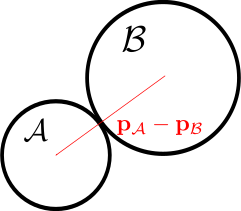
\includegraphics[height=.25\linewidth]{balls_touching}
        \end{figure}
        \begin{itemize}
            \item $|| \pA - \pB || = r_\A + r_\B \Rightarrow $ collision.
            \item normale de contact: $\frac{\pA - \pB}{|| \pA - \pB ||}$.
            \item point de contact: $\pB + \n * r_\B$.
        \end{itemize}
    }
    \only<4> {
        \framesubtitle{Cas de la pénétration}
        \begin{figure}[h]
            \includegraphics[height=.25\linewidth]{ball}
        \end{figure}
        \begin{itemize}
            \item $|| \pA - \pB || < r_\A + r_\B \Rightarrow $ pénétration.\\
            \item Profondeur de pénétration: $r_\A + r_\B - || \pA - \pB ||$.
        \end{itemize}
    }
    \end{overlayarea}
    }

\end{frame}

\begin{frame}[fragile]{Algo: objet convexe vs. plan}
    \begin{block}{Problème}
        Soit $\A$ une partie convexe de $\mathbb{R}^n$, et
        $\mathcal{P}$ un plan (demi-espace) de normale $\n$ et de position $\p$.
        Calculer l’éventuelle collision.
    \end{block}
    \only<2-> {
    \begin{overlayarea}{10cm}{10cm}
    \begin{description}
        \item
        \only<2> {
            \framesubtitle{Notion de convexité}
            \item[Convexité:]
                $\forall \pone, \ptwo \in \A^2, \lambda \in [0, 1], \lambda *
                \pone + (1 - \lambda) * \ptwo \in \A$
                \begin{figure}[h]
                    \setcounter{subfigure}{0}
                    \subfigure[Convexe]{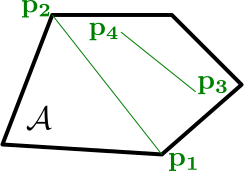
\includegraphics[height=.25\linewidth]{convexe}}
                    \subfigure[Concave]{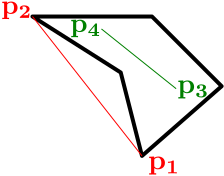
\includegraphics[height=.25\linewidth]{concave}}
                \end{figure}
        }
\end{description}
       \only<3> {
            \framesubtitle{Cas de la séparation}
           \begin{center}
               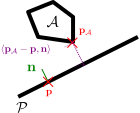
\includegraphics[height=.25\linewidth]{convex_vs_plan_nocolide}
           \end{center}
           \begin{itemize}
               \item $\left< \pA - \p, \n \right> > 0 \Rightarrow$ pas de collision.
               \item on ne sais pas (pour le moment) trouver $\pA$\ldots
           \end{itemize}
       }
       \only<4> {
            \framesubtitle{Cas du contact}
           \begin{center}
               \includegraphics[height=.25\linewidth]{convex_vs_plan_contact}
           \end{center}
           \begin{itemize}
               \item $\left< \pA - \p, \n \right> = 0 \Rightarrow$ pénétration.
               \item normale de contact: $\n$.
               \item point de contact: $\pA$.
           \end{itemize}
       }
       \only<5> {
            \framesubtitle{Cas de la pénétration}
           \begin{center}
               \includegraphics[height=.25\linewidth]{convex_vs_plan_penetration}
           \end{center}
           \begin{itemize}
               \item $\left< \pA - \p, \n \right> < 0 \Rightarrow$ pénétration.
               \item Profondeur de pénétration: $\left< \pA - \p, \n\right>$.
           \end{itemize}
       }
   %\begin{description}
       %\item
        \only<6> {
            \framesubtitle{Déterminer $\pA = s_\A(-\n)$}
        %\item[Fonction de support:]\mbox{}\\
                \begin{itemize}
                    \item On définit la \textbf{fonction de support} $s_\A(\v)$
                        de $\A$:
                        \[
                            s_\A(\v) = \argmax\limits_{\p \in \A} \left< \p, \v \right>
                        \]
                \end{itemize}
                \begin{center}
                    \includegraphics[height=.25\linewidth]{support_fun}
                \end{center}
        }
        \only<7> {
            \framesubtitle{Algorithme final}
            \begin{algorithm}[H]
            \begin{algorithmic}[1]
                \STATE $\pA  = s_\A(-\n)$
                \STATE $d = \left< \pA - p, n \right>$
                \IF{$d > 0$}
                    \RETURN Pas de collision.
                \ENDIF
                \RETURN (normal: $\n$, point: $\pA - \n * d$, pénétration: $d$)
            \end{algorithmic}
            \end{algorithm}
                \begin{center}
                    \includegraphics[height=.15\linewidth]{convex_vs_plan_penetration}
                \end{center}
        }
    \end{overlayarea}
    }
    %\end{description}
\end{frame}

\begin{frame}{Théorie: objet convexe vs. objet convexe}
    \begin{block}{Problème}
        Soient $\A$ et $\B$ deux parties convexes de
        $\mathbb{R}^n$, trouver $\pii \in \A$ et $\pj \in
        \B$, tels que $|| \pii - \pj || = 0$.
    \end{block}
    \only<2-> {
        \framesubtitle{La somme de Minkowski}
    \begin{overlayarea}{10cm}{10cm}
    \only<2-4> {
    \begin{itemize}
        \item<2-4> Soit $\A \oplus -\B = \{ \pii + (-\pj) \mid \pii \in
            \A \text{ et } \pj \in \B \}$\\
            Deux objets sont en collision ssi $0_{\mathbb{R}^n} \in
            \A \oplus -\B$.
        \item<3-4> Les points les plus proches entre $\A$ et
            $\B$ sont donnés par: \[ \argmin\limits_{\pii \in
            \A, \pj \in \B} || \pii - \pj || \]
        \item<4> La plus petite distance est donnée par \ldots
            \[ \min\limits_{\pii \in \A,
            \pj \in \B} || \pii - \pj || \]
            \ldots c’est à dire la distance entre $\A \oplus
            -\B$ et l’origine~!
    \end{itemize}
    }
    \only<5> {
    \begin{itemize}
        \item l’opération $\A \oplus \B$ s’apelle la
            \textbf{Somme de Minkowski} de $\A$ et $\B$.
        \item $\A \oplus - \B$ s’apelle le
            \textbf{Configuration Space Obstacle} (CSO).
        \item Le CSO est très lourd à calculer explicitement.
        \item Hereusement, certains algorithmes n’ont pas besoin d’un CSO explicite!
    \end{itemize}
    }
    \end{overlayarea}
    }
\end{frame}

\begin{frame}{Algo: objet convexe vs. objet convexe}
\end{frame}

\begin{frame}{Impliquant des objets concaves}
\end{frame}

\begin{frame}{Le calcul des forces}
\end{frame}
